\documentclass[10pt]{beamer}\usepackage[]{graphicx}\usepackage[]{color}
%% maxwidth is the original width if it is less than linewidth
%% otherwise use linewidth (to make sure the graphics do not exceed the margin)
\makeatletter
\def\maxwidth{ %
  \ifdim\Gin@nat@width>\linewidth
    \linewidth
  \else
    \Gin@nat@width
  \fi
}
\makeatother

\definecolor{fgcolor}{rgb}{0.345, 0.345, 0.345}
\newcommand{\hlnum}[1]{\textcolor[rgb]{0.686,0.059,0.569}{#1}}%
\newcommand{\hlstr}[1]{\textcolor[rgb]{0.192,0.494,0.8}{#1}}%
\newcommand{\hlcom}[1]{\textcolor[rgb]{0.678,0.584,0.686}{\textit{#1}}}%
\newcommand{\hlopt}[1]{\textcolor[rgb]{0,0,0}{#1}}%
\newcommand{\hlstd}[1]{\textcolor[rgb]{0.345,0.345,0.345}{#1}}%
\newcommand{\hlkwa}[1]{\textcolor[rgb]{0.161,0.373,0.58}{\textbf{#1}}}%
\newcommand{\hlkwb}[1]{\textcolor[rgb]{0.69,0.353,0.396}{#1}}%
\newcommand{\hlkwc}[1]{\textcolor[rgb]{0.333,0.667,0.333}{#1}}%
\newcommand{\hlkwd}[1]{\textcolor[rgb]{0.737,0.353,0.396}{\textbf{#1}}}%
\let\hlipl\hlkwb

\usepackage{framed}
\makeatletter
\newenvironment{kframe}{%
 \def\at@end@of@kframe{}%
 \ifinner\ifhmode%
  \def\at@end@of@kframe{\end{minipage}}%
  \begin{minipage}{\columnwidth}%
 \fi\fi%
 \def\FrameCommand##1{\hskip\@totalleftmargin \hskip-\fboxsep
 \colorbox{shadecolor}{##1}\hskip-\fboxsep
     % There is no \\@totalrightmargin, so:
     \hskip-\linewidth \hskip-\@totalleftmargin \hskip\columnwidth}%
 \MakeFramed {\advance\hsize-\width
   \@totalleftmargin\z@ \linewidth\hsize
   \@setminipage}}%
 {\par\unskip\endMakeFramed%
 \at@end@of@kframe}
\makeatother

\definecolor{shadecolor}{rgb}{.97, .97, .97}
\definecolor{messagecolor}{rgb}{0, 0, 0}
\definecolor{warningcolor}{rgb}{1, 0, 1}
\definecolor{errorcolor}{rgb}{1, 0, 0}
\newenvironment{knitrout}{}{} % an empty environment to be redefined in TeX

\usepackage{alltt}%
\usetheme{Boadilla}
\usecolortheme{seahorse}

\usepackage[utf8]{inputenc}%

% graphics
%% Figures %%%%%%%%%%%%%%%%%%%%%%%%%%%%%%%%%%%%%%%%%%%%%%%%%%
\usepackage{graphicx}
\usepackage{xcolor}%for color mixing

\usepackage{amsmath}%
\usepackage{amsfonts}%
\usepackage{amssymb}%
\usepackage{graphicx}

%%%%%%%%%%%%%%%%%%%%%%%%%%%%%%%%%%%%%%%%%%%%%%
%%%%%%%%%%%%%%%%% Doc info %%%%%%%%%%%%%%%%%%%
\title[\textbf{Intro to R}]{Introduction to R}
\date{\today}

%%%%%%%%%%%%%%%%%%%%%%%%%%%%%%%%%%%%%%%%%%%%%%
\IfFileExists{upquote.sty}{\usepackage{upquote}}{}
\begin{document}



\begin{frame}
\maketitle	
\end{frame}
%%%%%%%%%%%

\begin{frame}{R and RStudio}
  \begin{center}
    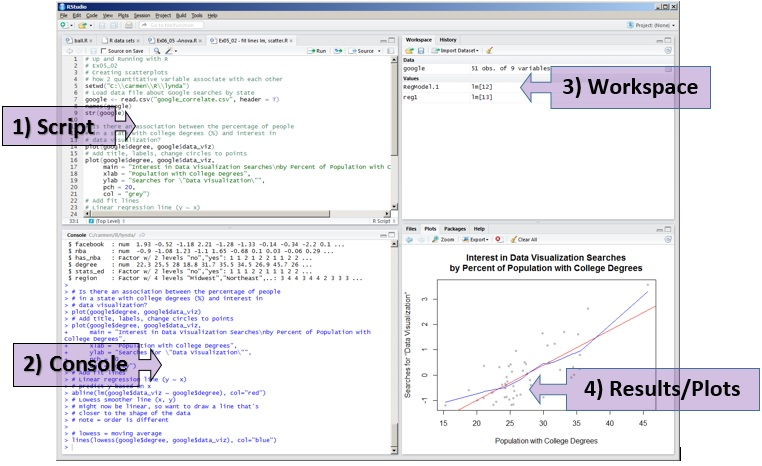
\includegraphics[width=0.8\textwidth]{Figures/rstudiolayout}
  \end{center}
\end{frame}
%%%%%%%%%%%

\begin{frame}{What R can do}

  \pause \begin{exampleblock}{Everything.$^{1,2}$}
    
  {\tiny $1$ Except think about your science}\\
  {\tiny $2$ Occasionally in a non efficient way}
  \end{exampleblock}
  
  \pause \begin{block}{What about RStudio?}
  Make your life easier\\
  Many handy tricks.
  \end{block}
\end{frame}
%%%%%%%%%%%

\AtBeginSection[]
{
  \begin{frame}<beamer>
    \frametitle{}
    \tableofcontents[currentsection,hideothersubsections,subsectionstyle=hide]% down vote\tableofcontents[currentsection,currentsubsection,hideothersubsections,sectionstyle=show/hide,subsectionstyle=show/shaded/hide] 
  \end{frame}
} 
\section{The mean}

\begin{frame}[fragile]{Calculating a mean: Arithmetic and assignment}

\begin{knitrout}
\definecolor{shadecolor}{rgb}{0.843, 0.867, 0.922}\color{fgcolor}\begin{kframe}
\begin{alltt}
  \hlstd{(}\hlnum{2} \hlopt{+} \hlnum{3} \hlopt{+} \hlnum{5} \hlopt{+} \hlnum{1}\hlstd{)} \hlopt{/} \hlnum{4}
\end{alltt}
\begin{verbatim}
[1] 2.75
\end{verbatim}
\end{kframe}
\end{knitrout}
\pause
\begin{knitrout}
\definecolor{shadecolor}{rgb}{0.843, 0.867, 0.922}\color{fgcolor}\begin{kframe}
\begin{alltt}
  \hlstd{a} \hlkwb{<-} \hlnum{2}
  \hlstd{b} \hlkwb{<-} \hlnum{3}
  \hlstd{c} \hlkwb{<-} \hlnum{5}
  \hlstd{d} \hlkwb{<-} \hlnum{1}

  \hlstd{(a} \hlopt{+} \hlstd{b} \hlopt{+} \hlstd{c} \hlopt{+} \hlstd{d)} \hlopt{/} \hlnum{4}
\end{alltt}
\begin{verbatim}
[1] 2.75
\end{verbatim}
\end{kframe}
\end{knitrout}
\pause
\begin{knitrout}
\definecolor{shadecolor}{rgb}{0.843, 0.867, 0.922}\color{fgcolor}\begin{kframe}
\begin{alltt}
  \hlstd{a} \hlkwb{<-} \hlnum{45}
  \hlstd{(a} \hlopt{+} \hlstd{b} \hlopt{+} \hlstd{c} \hlopt{+} \hlstd{d)} \hlopt{/} \hlnum{4}
\end{alltt}
\begin{verbatim}
[1] 13.5
\end{verbatim}
\end{kframe}
\end{knitrout}
\end{frame}
%%%%%%%%%%%


\begin{frame}[fragile]{Calculating a mean: using vectors} % tiring to type again and again
\begin{knitrout}
\definecolor{shadecolor}{rgb}{0.843, 0.867, 0.922}\color{fgcolor}\begin{kframe}
\begin{alltt}
\hlkwd{c}\hlstd{(}\hlnum{2}\hlstd{,}\hlnum{3}\hlstd{,}\hlnum{5}\hlstd{,}\hlnum{1}\hlstd{)} \hlcom{# c is for concatenate}
\end{alltt}
\begin{verbatim}
[1] 2 3 5 1
\end{verbatim}
\end{kframe}
\end{knitrout}
  \pause
\begin{knitrout}
\definecolor{shadecolor}{rgb}{0.843, 0.867, 0.922}\color{fgcolor}\begin{kframe}
\begin{alltt}
\hlstd{mydata} \hlkwb{<-} \hlkwd{c}\hlstd{(}\hlnum{2}\hlstd{,}\hlnum{3}\hlstd{,}\hlnum{5}\hlstd{,}\hlnum{1}\hlstd{)} \hlcom{# save the vector}
\end{alltt}
\end{kframe}
\end{knitrout}
  \pause
  
\begin{knitrout}
\definecolor{shadecolor}{rgb}{0.843, 0.867, 0.922}\color{fgcolor}\begin{kframe}
\begin{alltt}
 mydata <- (2,3,5,1) \hlcom{# c is missing => error!}
\end{alltt}


{\ttfamily\noindent\bfseries\color{errorcolor}{Error: <text>:1:14: unexpected ','\\1:\ \ mydata <- (2,\\\ \ \ \ \ \ \ \ \ \ \ \ \ \ \ \  \textasciicircum{}}}\end{kframe}
\end{knitrout}
  
  \pause
  
  Why bother with vectors?
\begin{knitrout}
\definecolor{shadecolor}{rgb}{0.843, 0.867, 0.922}\color{fgcolor}\begin{kframe}
\begin{alltt}
  \hlstd{mydata[}\hlnum{2}\hlstd{]} \hlkwb{<-} \hlnum{4}
  \hlstd{mydata}
\end{alltt}
\begin{verbatim}
[1] 2 4 5 1
\end{verbatim}
\end{kframe}
\end{knitrout}
\end{frame}
%%%%%%%%%%%

\begin{frame}[fragile]{Calculating a mean: using functions}%shortcut
  
  How to use a function?
\begin{knitrout}
\definecolor{shadecolor}{rgb}{0.843, 0.867, 0.922}\color{fgcolor}\begin{kframe}
\begin{alltt}
  \hlopt{?}\hlstd{mean}
\end{alltt}
\end{kframe}
\end{knitrout}
  
\pause

\begin{knitrout}
\definecolor{shadecolor}{rgb}{0.843, 0.867, 0.922}\color{fgcolor}\begin{kframe}
\begin{alltt}
\hlkwd{mean}\hlstd{(}\hlkwd{c}\hlstd{(}\hlnum{2}\hlstd{,}\hlnum{4}\hlstd{,}\hlnum{5}\hlstd{,}\hlnum{1}\hlstd{))}
\end{alltt}
\begin{verbatim}
[1] 3
\end{verbatim}
\begin{alltt}
\hlkwd{mean}\hlstd{(mydata)}
\end{alltt}
\begin{verbatim}
[1] 3
\end{verbatim}
\begin{alltt}
\hlkwd{mean}\hlstd{(}\hlkwc{x} \hlstd{= mydata)}
\end{alltt}
\begin{verbatim}
[1] 3
\end{verbatim}
\end{kframe}
\end{knitrout}
  

\end{frame}
%%%%%%%%%%%

%%%%%%%%%%%%%%%%%%%%%%%%%%%%%%%%%%%%%%%%%%%%%%%%%%%%%%%%%%%%%%%%%%%%%%%%%%%%%%%%%
\section{Working with 2D objects}

\begin{frame}[fragile]{Loading data}
  
\begin{knitrout}
\definecolor{shadecolor}{rgb}{0.843, 0.867, 0.922}\color{fgcolor}\begin{kframe}
\begin{alltt}
  \hlkwd{data}\hlstd{(}\hlstr{"trees"}\hlstd{)}
\end{alltt}
\end{kframe}
\end{knitrout}
  \pause
  
\begin{knitrout}
\definecolor{shadecolor}{rgb}{0.843, 0.867, 0.922}\color{fgcolor}\begin{kframe}
\begin{alltt}
\hlkwd{str}\hlstd{(trees)}
\end{alltt}
\begin{verbatim}
'data.frame':	31 obs. of  3 variables:
 $ Girth : num  8.3 8.6 8.8 10.5 10.7 10.8 11 11 11.1 11.2 ...
 $ Height: num  70 65 63 72 81 83 66 75 80 75 ...
 $ Volume: num  10.3 10.3 10.2 16.4 18.8 19.7 15.6 18.2 22.6 19.9 ...
\end{verbatim}
\end{kframe}
\end{knitrout}
  
  Try also \texttt{summary}, \texttt{class}, \texttt{head}, \texttt{tail}
\end{frame}
%%%%%%%%%%%



%%%%%%%%%%%%%%%%%%%%%%%%%%%%%%%%%%%%%%%%%%%%%%%%%%%%%%%%%%%%%%%%%%%%%%%%%%%%%%%%%
%%%%%%%%%%%%%%%%%%%%%%%%%%%%%%%%%%%%%%%%%%%%%%%%%%%%%%%%%%%%%%%%%%%%%%%%%%%%%%%%%
\section{T-test}

\begin{frame}[fragile]{Student's T.test introduction}% presenting the test, the output...
\begin{knitrout}
\definecolor{shadecolor}{rgb}{0.843, 0.867, 0.922}\color{fgcolor}\begin{kframe}
\begin{alltt}
\hlopt{?}\hlstd{t.test}
\end{alltt}
\end{kframe}
\end{knitrout}
  
  \pause
\begin{knitrout}
\definecolor{shadecolor}{rgb}{0.843, 0.867, 0.922}\color{fgcolor}\begin{kframe}
\begin{alltt}
\hlkwd{t.test}\hlstd{(}\hlnum{1}\hlopt{:}\hlnum{10}\hlstd{,} \hlkwc{y} \hlstd{=} \hlkwd{c}\hlstd{(}\hlnum{7}\hlopt{:}\hlnum{20}\hlstd{))}
\end{alltt}
\begin{verbatim}

	Welch Two Sample t-test

data:  1:10 and c(7:20)
t = -5.4349, df = 21.982, p-value = 1.855e-05
alternative hypothesis: true difference in means is not equal to 0
95 percent confidence interval:
 -11.052802  -4.947198
sample estimates:
mean of x mean of y 
      5.5      13.5 
\end{verbatim}
\end{kframe}
\end{knitrout}
  
\end{frame}
%%%%%%%%%%%

\begin{frame}[fragile]{T.test introduction}% presenting the test, the output...

\begin{knitrout}
\definecolor{shadecolor}{rgb}{0.843, 0.867, 0.922}\color{fgcolor}\begin{kframe}
\begin{alltt}
  \hlkwd{boxplot}\hlstd{(}\hlkwd{c}\hlstd{(}\hlnum{1}\hlopt{:}\hlnum{10}\hlstd{,} \hlnum{7}\hlopt{:}\hlnum{20}\hlstd{)} \hlopt{~} \hlkwd{c}\hlstd{(}\hlkwd{rep}\hlstd{(}\hlnum{1}\hlstd{,}\hlnum{10}\hlstd{),} \hlkwd{rep}\hlstd{(}\hlnum{2}\hlstd{,} \hlnum{14}\hlstd{)))}
\end{alltt}
\end{kframe}
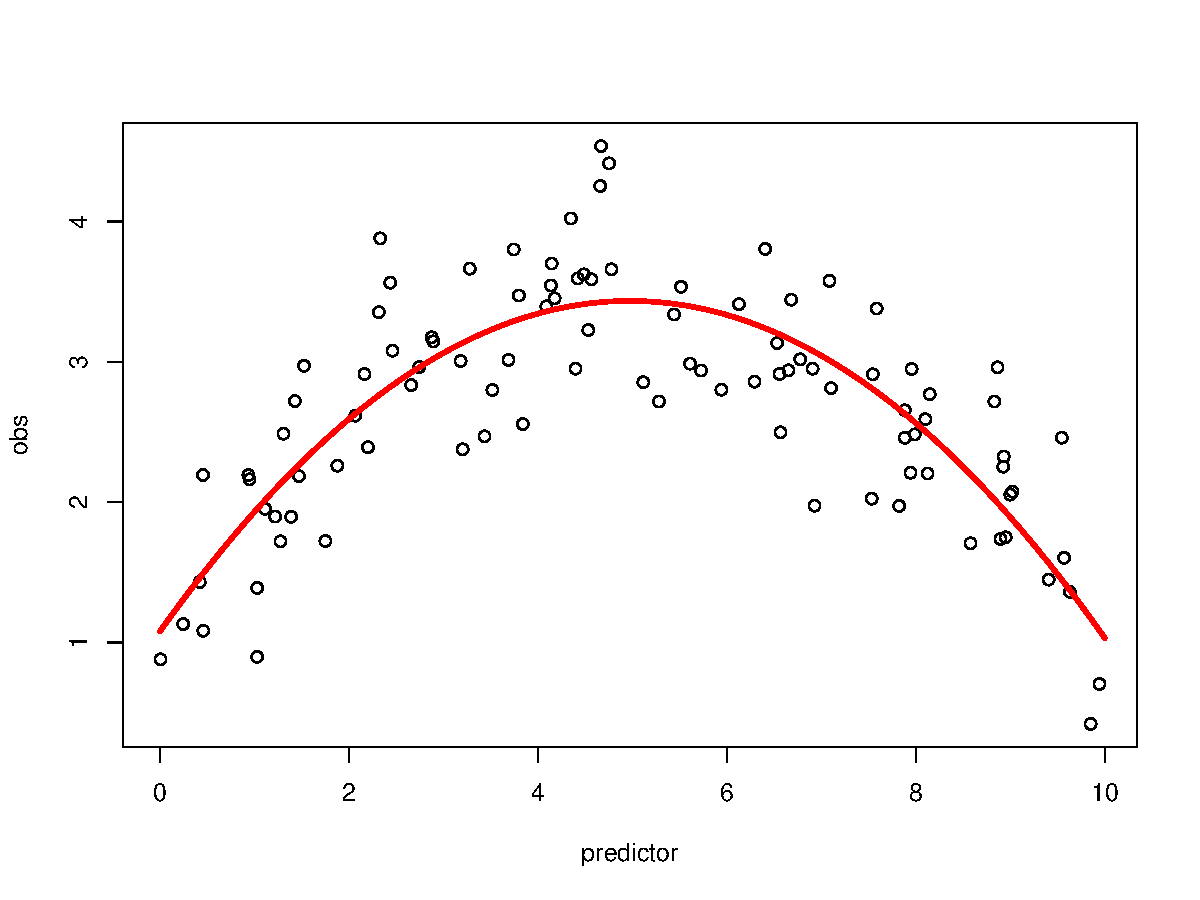
\includegraphics[width=0.8\textwidth,height=0.6\textwidth]{figure/unnamed-chunk-14-1} 

\end{knitrout}
\end{frame}
%%%%%%%%%%%


\section{Open problem}

\begin{frame}[fragile]{The t.test problem}
  
\begin{knitrout}
\definecolor{shadecolor}{rgb}{0.843, 0.867, 0.922}\color{fgcolor}\begin{kframe}
\begin{alltt}
\hlkwd{t.test}\hlstd{(}\hlnum{1}\hlopt{:}\hlnum{10}\hlstd{,} \hlkwc{y} \hlstd{=} \hlkwd{c}\hlstd{(}\hlnum{2}\hlopt{:}\hlnum{20}\hlstd{,}\hlopt{-}\hlnum{9}\hlstd{),} \hlkwc{var.equal} \hlstd{=} \hlnum{FALSE}\hlstd{)}
\end{alltt}
\begin{verbatim}

	Welch Two Sample t-test

data:  1:10 and c(2:20, -9)
t = -2.4345, df = 27.642, p-value = 0.02163
alternative hypothesis: true difference in means is not equal to 0
95 percent confidence interval:
 -8.2885317 -0.7114683
sample estimates:
mean of x mean of y 
      5.5      10.0 
\end{verbatim}
\end{kframe}
\end{knitrout}
\end{frame}
%%%%%%%%%%%

\begin{frame}[fragile]{The t.test problem}
\begin{knitrout}
\definecolor{shadecolor}{rgb}{0.843, 0.867, 0.922}\color{fgcolor}\begin{kframe}
\begin{alltt}
\hlkwd{t.test}\hlstd{(}\hlnum{1}\hlopt{:}\hlnum{10}\hlstd{,} \hlkwc{y} \hlstd{=} \hlkwd{c}\hlstd{(}\hlnum{2}\hlopt{:}\hlnum{20}\hlstd{,}\hlopt{-}\hlnum{9}\hlstd{),} \hlkwc{var.equal} \hlstd{=} \hlnum{TRUE}\hlstd{)}
\end{alltt}
\begin{verbatim}

	Two Sample t-test

data:  1:10 and c(2:20, -9)
t = -1.9134, df = 28, p-value = 0.06597
alternative hypothesis: true difference in means is not equal to 0
95 percent confidence interval:
 -9.3175688  0.3175688
sample estimates:
mean of x mean of y 
      5.5      10.0 
\end{verbatim}
\end{kframe}
\end{knitrout}
 
\end{frame}
%%%%%%%%%%%

\begin{frame}[fragile]{The t.test problem}
  Random sample from a Gaussian distribution with variance 1
\begin{knitrout}
\definecolor{shadecolor}{rgb}{0.843, 0.867, 0.922}\color{fgcolor}\begin{kframe}
\begin{alltt}
  \hlkwd{set.seed}\hlstd{(}\hlkwc{seed} \hlstd{=} \hlnum{179}\hlstd{)}
  \hlstd{x1} \hlkwb{<-} \hlkwd{rnorm}\hlstd{(}\hlkwc{n} \hlstd{=} \hlnum{20}\hlstd{,} \hlkwc{mean} \hlstd{=} \hlnum{0}\hlstd{,} \hlkwc{sd} \hlstd{=} \hlnum{1}\hlstd{)}
  \hlstd{x2} \hlkwb{<-} \hlkwd{rnorm}\hlstd{(}\hlkwc{n} \hlstd{=} \hlnum{20}\hlstd{,} \hlkwc{mean} \hlstd{=} \hlnum{0}\hlstd{,} \hlkwc{sd} \hlstd{=} \hlnum{1}\hlstd{)}


  \hlkwd{var}\hlstd{(x1)}
\end{alltt}
\begin{verbatim}
[1] 0.7040416
\end{verbatim}
\begin{alltt}
  \hlkwd{var}\hlstd{(x2)}
\end{alltt}
\begin{verbatim}
[1] 1.810404
\end{verbatim}
\end{kframe}
\end{knitrout}
\end{frame}
%%%%%%%%%%%

\begin{frame}[fragile]{The t.test problem}
\begin{knitrout}
\definecolor{shadecolor}{rgb}{0.843, 0.867, 0.922}\color{fgcolor}\begin{kframe}
\begin{alltt}
  \hlkwd{var.test}\hlstd{(}\hlkwc{x} \hlstd{= x1,} \hlkwc{y} \hlstd{= x2)}
\end{alltt}
\begin{verbatim}

	F test to compare two variances

data:  x1 and x2
F = 0.38889, num df = 19, denom df = 19, p-value = 0.04593
alternative hypothesis: true ratio of variances is not equal to 1
95 percent confidence interval:
 0.1539260 0.9825028
sample estimates:
ratio of variances 
         0.3888866 
\end{verbatim}
\end{kframe}
\end{knitrout}
  \textbf{Should we use var.equal = TRUE or FALSE ?\\}
  
  \textbf{When var.test significant/not?}
\end{frame}
%%%%%%%%%%%

\begin{frame}{}

\end{frame}
%%%%%%%%%%%
\begin{frame}{Bonus open problems if you get bored}

  
\end{frame}
  
\end{document}
